\section*{Phần 10.4}
\subsection*{Bài 2}
Mỗi danh sách đỉnh sau đây có lập thành một đường đi trong đồ thị dưới đây không? Những đường đi nào là đơn giản? Đâu là chu trình? Độ dài của những đường đi đó là bao nhiêu?
\begin{enumerate}[label=\alph*)]
    \item a, b, e, c, b
    \item a, d, a, d, a
    \item a, d, b, e, a
    \item a, b, e, c, b, d, a
\end{enumerate}
\begin{center}
    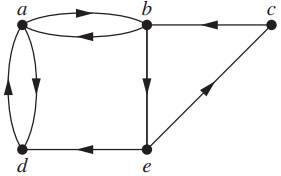
\includegraphics[scale=0.75]{10.4_2.png}
\end{center}
\begin{proof}.
    \begin{enumerate}[label=\alph*)]
        \item Kiểm tra các cặp đỉnh liên tiếp nhau đều tồn tại đường đi giữa chúng, vậy đây là một đường đi độ dài 5.
        \item Kiểm tra các cặp đỉnh liên tiếp nhau đều tồn tại đường đi giữa chúng, vậy đây là một đường đi độ dài 5.
        \item Vì không có đường đi giữa d và b nên đây không phải đường đi hợp lệ.
        \item Vì không có đường đi giữa b và d nên đây không phải đường đi hợp lệ.
    \end{enumerate}
\end{proof}
\subsection*{Bài 6}
Có bao nhiêu thành phần liên thông trong các đồ thị từ bài 3 đến bài 5? Với mỗi đồ thị hãy tìm từng thành phần liên thông.
\begin{center}
    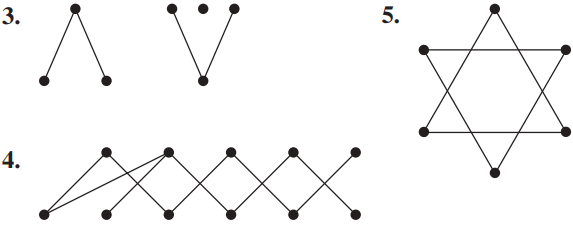
\includegraphics[scale=0.5]{10.4_6.png}
\end{center}
\begin{proof}
    Bài 3 có 3 thành phần liên thông, 1 là 3 đỉnh xếp thành hình chữ A, 2 là 3 đỉnh xếp thành hình chữ V và 3 là một đỉnh ở giữa chữ V đó, các thành phần này không có cạnh nào nối chúng với nhau. Bài 4 và 5 chỉ có một thành phần vì tất cả các đỉnh đều được nối với nhau.
\end{proof}
\subsection*{Bài 16}
Chứng minh rằng nếu $G=(V, E)$ là một đồ thị có hướng và $u$, $v$, và $w$ là các đỉnh trong $V$ với $u$ và $v$ đều có thể đến được nhau, và $v$ và $w$ đều có thể đến được nhau, thì $u$ và $w$ có thể đến được nhau.
\begin{proof}
	Nếu $u$ và $v$ đều có thể đến được nhau trong một đồ thị có hướng, vậy có đường đi từ $u$ đến $v$ và ngược lại, ta có thể coi 2 cạnh này như một cạnh vô hướng. Vậy theo tính chất bắc cầu, nếu có một cạnh vô hướng từ $u$ đến $v$, và có một cạnh vô hướng từ $v$ đến $w$ thì sẽ có đường đi vô hướng từ $u$ đến $w$.
\end{proof}
\subsection*{Bài 19}
Tìm số đường đi độ dài $n$ giữa hai đỉnh khác nhau của đồ thị $K_4$ nếu $n$ là
\begin{enumerate}[label=\alph*)]
	\begin{multicols}{4}
		\item 2
		\item 3
		\item 4
		\item 5
	\end{multicols}
\end{enumerate}
\begin{proof}.
\begin{enumerate}[label=\alph*)]
	\item Một đường đi độ dài 2 có dạng $a_1,a_2,a_3$. Vì $a_1\neq a_2$, ta có $a_3$ có thể là 3 đỉnh còn lại, vậy ta được $A^2_4\cdot3=36$ đường.
	\item Đường đi này bao gồm 36 đường đi $a_1,a_2,a_3$ và một điểm $a_4$. Vì $a_4\neq a_3$, ta lại có $a_4$ có thể là 3 đỉnh còn lại, ta được $36\cdot3=108$ đường đi.
	\item Tương tự như câu trên, ta có 324 đường đi.
	\item Tương tự như câu trên, ta có 972 đường đi.
\end{enumerate}
\end{proof}
\subsection*{Bài 20}
Dùng đường đi để chứng minh rằng hai đồ thị sau không đồng phân với nhau hoặc tìm một đồng phân khác của chúng.
\begin{center}
	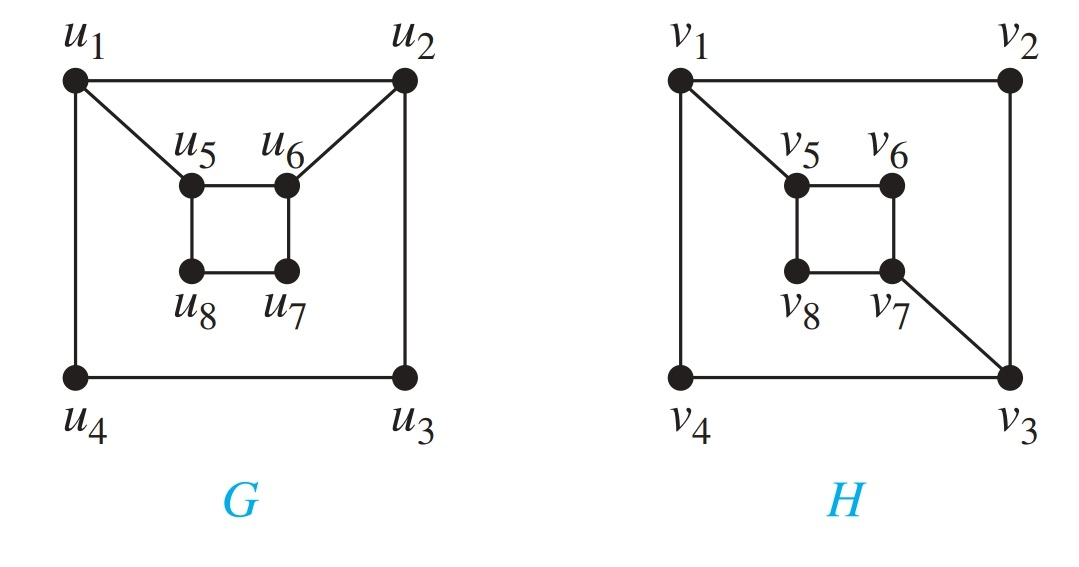
\includegraphics[scale=0.25]{10.4_20.jpg}
\end{center}
\begin{proof}
	Dễ thấy rằng ở đồ thị bên phải ta có đường đi $v_1,v_5,v_8,v_7,v_3$ độ dài 4, ta không thể tìm được đường đi qua các cạnh tương đương ở đồ thị bên trái. Vậy hai đồ thị trên không đồng phân với nhau.
\end{proof}
\subsection*{Bài 28}
Chứng minh rằng một đồ thị liên thông $n$ đỉnh cần ít nhất $n-1$ cạnh.
\begin{proof}
Cho $n$ đỉnh rời rạc với nhau. Vì một cạnh nối 2 đỉnh, ta sẽ lần lượt chọn 1 đỉnh bất kì, nối với 1 đỉnh khác chưa được nối bất kì cạnh nào. Cứ sau 1 lượt, số đỉnh chưa được kết nối giảm 1. Riêng lượt đầu tiên số đỉnh này giảm 2, suy ra sẽ có $n-1$ lượt, vậy có $n-1$ cạnh, suy ra điều phải chứng minh.
\end{proof}
\subsection*{Bài 35}
Cho rằng $v$ là đầu mút của một cạnh cầu. Chứng minh rằng $v$ là một đỉnh cắt nếu $v$ không phải là đỉnh treo.
\begin{proof}
Ta biết rằng, một cạnh cầu nối hai thành phần liên thông, nghĩa là nối 2 đỉnh bất kì của 2 thành phần đó. Vậy với 2 đỉnh đó, nó phải từ bậc 2 trở lên vì nó nối với cạnh cầu và nối với thành phần liên thông của nó. Chứng minh theo chiều ngược lại, nếu đỉnh này là đỉnh treo (bậc 1), nó chỉ nối với thành phần liên thông, hoặc với cạnh cầu, bỏ đi đỉnh đó và cạnh cầu đó không làm tăng số thành phần liên thông, suy ra điều phải chứng minh.
\end{proof}
\subsection*{Bài 36}
Chứng minh rằng đỉnh $c$ trong một đồ thị liên thông G là một đỉnh cắt nếu tồn tại đỉnh $u,v\neq c$ sao cho mọi đường đi từ $u$ đến $v$ phải qua $c$.
\begin{proof}
Nếu $u,v$ cùng thuộc một thành phần liên thông trong G thì luôn tồn tại đường đi từ $u$ đến $v$. Vậy suy ra ta phải chọn $u$ và $v$ trong hai thành phần liên thông khác nhau được nối bởi $c$, hay $c$ là đỉnh cắt của đồ thị.
\end{proof}
\subsection*{Bài 38}
Chứng minh rằng một đồ thị ít nhất 2 đỉnh phải có ít nhất 2 đỉnh không phải là đỉnh cắt.
\begin{proof}
Ta biết đỉnh cắt nối 2 thành phần liên thông với nhau. Một thành phần liên thông có thể là một đồ thị, hoặc có thể chỉ là một đỉnh. Vì vậy, hai đỉnh này không thể là đỉnh cắt, trong trường hợp đơn giản nhất. Nếu có nhiều đỉnh hơn, chúng cũng không thể là đỉnh cắt vì nằm cùng trong một thành phần liên thông. Nếu đồ thị chỉ có 2 đỉnh và 1 cạnh, đương nhiên nó không phải đỉnh cắt, vì chỉ có 1 thành phần liên thông, không thể tạo ra đỉnh cắt, suy ra điều phải chứng minh.
\end{proof}